Se ha concentrado en la~\autoref{aportes} una serie de aportes que se consideran
importantes en la literatura, relacionados con la aplicación de algoritmos de
\hyperlink{abbr}{IA} en el área médica. La propuesta de esta tesis cumple con
todos excepto con la realización de una revisión de literatura, cumpliendo un
requisito extra: el despliegue en hardware.

\begin{table}[H]
    \centering
    \resizebox{\textwidth}{!}{%
    \begin{tabular}{@{} cl*{12}c @{}}
     & \rot{\shortstack[l]{Análisis de \\imagen}} & \rot{\shortstack[l]{Emisión
    de \\diagnóstico}} & \rot{\shortstack[l]{Inteligencia artificial\\en
    medicina}} & \rot{\shortstack[l]{Sistemas de diagnóstico \\ asistido por computadora}} & \rot{\shortstack[l]{Big
    data}} & \rot{\shortstack[l]{Revisión de\\literatura}} &
    \rot{\shortstack[l]{Procesamiento digital\\de imágenes}} &
    \rot{\shortstack[l]{Aprendizaje\\automatizado}} &
    \rot{\shortstack[l]{Aprendizaje\\profundo}} &
    \rot{\shortstack[l]{Redes\\neuronales}} & \rot{\shortstack[l]{Redes
    neuronales\\convolucionadas}} & \rot{\shortstack[l]{Despliegue\\en
    hardware}} \\ \midrule 1 & \OK & \OK & \OK & \OK & \OK &  & \OK & & \OK &  &
    \OK &  &  \\
    2 &  & \OK & \OK & \OK &  &  & \OK &  & \OK &  & \OK &  &  \\
    3 &  & \OK & \OK & \OK &  &  &  &  & \OK & \OK &  &  &  \\
    4 & \OK & \OK & \OK & \OK &  &  &  & \OK & \OK &  & \OK &  &  \\
    5 &  & \OK & \OK & \OK &  & \OK & \OK & \OK & \OK &  &  &  &  \\
    6 & \OK & \OK & \OK & \OK & \OK &  & \OK & \OK & \OK & \OK & \OK & \OK &  \\
    7 &  & \OK & \OK & \OK &  &  &  & \OK & \OK &  &  &  &  \\
    8 & \OK &  &  & \OK &  & \OK &  &  &  &  &  &  &  \\
    9 & \OK &  & \OK & \OK &  &  &  &  & \OK & \OK &  &  &  \\
    10 &  &  & \OK & \OK &  &  &  &  & \OK & \OK & \OK & \OK &  \\
    11 & \OK & \OK & \OK &  &  &  & \OK & \OK & \OK & \OK & \OK & \OK &  \\
    \rot{\rlap{~~~~~~~Número de aporte}}
    Tesis & \OK & \OK & \OK & \OK & \OK & & \OK & \OK & \OK & \OK & \OK & \OK &
    \OK \\ 
    \bottomrule
    \end{tabular}%
    }
    \caption{Aportes y sus contribuciones}\label{aportes}
\end{table}

Así mismo, en comparación a cada uno de los trabajos aquí citados, la propuesta
ofrece mejor eficiencia en el desarrollo del \hyperlink{abbr}{SDAC} en
comparación con aquellos trabajos que usan \hyperlink{abbr}{ML}; el uso de las
\hyperlink{abbr}{ConvNet}s nos permite ahorrar dos pasos que eficiencia también
obedece a que las imágenes requieren muy poco tratamiento de
\hyperlink{abbr}{PDI} para poder ser alimentadas a la red para su clasificación.

Otra ventaja contra algunos aportes aquí presentados, es el uso de redes
previamente entrenadas para tareas generales de Visión por Computadora
(\hyperlink{abbr}{VC}\nomenclature{VC}{Visión por Computadora}), pudiendo
reentrenar tales redes para su aplicación en el diagnóstico médico. El
\hyperlink{abbr}{TL} es una forma poderosa de usar las
\hyperlink{abbr}{ConvNet}s y ahorrar en tiempo de entrenamiento y, lo más
importante, permite entrenar modelos con \hyperlink{abbr}{BD}s de tamaño modesto.

Como se expondrá posteriormente, los modelos presentados dentro de esta tesis
mejoran el rendimiento final, llegando a inclusive a duplicar el rendimiento
medido por la tasa de error comparado con otras aplicaciones similares de
\hyperlink{abbr}{ConvNets}s. Este rendimiento fue precisamente calculado
utilizando tres métricas de entrenamiento: exactitud, sensibilidad y
especificidad; la mayoría de los aportes expuestos utilizan solo una métrica de
entrenamiento.

La comprobación de supuestos realizada en esta tesis es algo que la distingue,
los trabajos previos carecen de esta fase. Para ello se utilizaron más de cuatro
técnicas de visualización, exploración y reducción de dimensionalidad para
extraer toda la información posible del comportamiento de los modelos.
Básicamente podemos ver exactamente que está observando la red para clasificar
las imágenes. La mayoría de las veces se toman a los algoritmos de DL como cajas
negras de las cuales se desconoce su comportamiento interno, aquí se pretende
esclarecer este comportamiento para mejorar la interpretabilidad de los modelos,
lo cual es sumamente importante en el área médica.

Mientras que los trabajos aquí presentados se limitan a pocas pruebas para medir
el poder de generalización del modelo y poder estimar su rendimiento real,
dentro de esta tesis podremos encontrar una batería completa de métricas de
evaluación que pretenden estimar con suma exactitud el poder total del algoritmo
para realizar la tarea de clasificación. Se tomó especial cuidado en todas las
consideraciones estadísticas, realizando complejos métodos de evaluación como la
validación cruzada de k iteraciones, lo que nos permite aseverar con mucha
certeza el rendimiento y capacidad de generalización del modelo.

El uso de una \hyperlink{abbr}{BD} previamente validada y que funge como patrón
para la evaluación de algoritmos aplicados a la clasificación de células en un
\hyperlink{abbr}{PAP} no solo ofrece los beneficios de tener una base sólida
sobre la cual entrenar el algoritmo. También nos permitió aplicar una técnica
jamás usada previamente sobre esta \hyperlink{abbr}{BD}, creando un aporte
novedoso al problema aquí atacado. La Segmentación Semántica nos permite saber
si un pixel determinado pertenece al fondo, al citoplasma o al núcleo de la
célula, lo cual lo hace una herramienta sumamente poderosa que pretende
solucionar el problema de segmentación y extracción de cada célula individual.

Por último, el paradigma de este trabajo orbita el concepto de aplicabilidad y
uso dentro del laboratorio. Se propone el trabajo conjunto entre el experto y el
\hyperlink{abbr}{SDAC} para alcanzar mejor rendimiento que cada uno de ellos de
manera individual. Los trabajos compilados utilizan un punto de vista más
enfocado a la investigación que a la aplicación real e inmediata de los modelos,
mediante el despliegue en hardware, nos aseguramos acercarnos más al objetivo
final que es el uso en el campo. Pensar el desarrollo como un sistema más que
como un modelo permitirá a futuro desarrollar maneras de extraer conocimiento
del experto en tiempo real para mejorar el rendimiento del
\hyperlink{abbr}{SDAC}, reentrenándose a si mismo de manera automática al mismo
tiempo que el utiliza y retroalimenta al sistema. 

El diseño conceptual estará enfocado a crear un dispositivo discreto de
hardware, para analizar muestras bajo microscopio. Capturando la imagen mediante
una cámara para posteriormente procesarla \emph{in-situ} dentro del laboratorio.
En la \autoref{fig:diagrama_sistema} podemos observar un bosquejo inicial de las
partes principales que integrarán el sistema.

\begin{figure}[H]
    \centering
    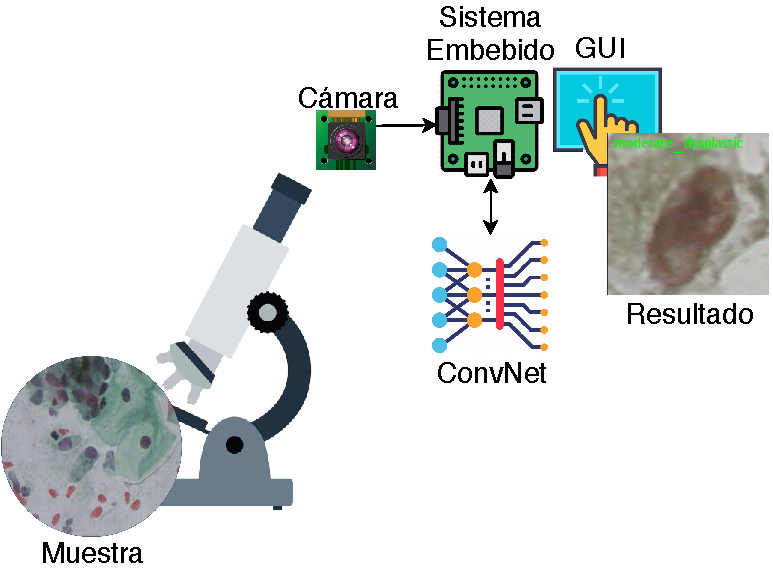
\includegraphics[width=0.6\textwidth]{capitulo_generalidades/diagrama_sistema}
    \caption{Diagrama del diseño conceptual}\label{fig:diagrama_sistema}
\end{figure}